\documentclass[a4paper]{article}

\usepackage{graphicx}
\usepackage{amsmath,amssymb}
\usepackage{minted}
\usepackage{multirow}
\usepackage{float}
\usepackage{algorithm}
\usepackage{algpseudocode}
\usepackage{todonotes}
\usepackage{forest}
\usepackage{xstring}
\usepackage{xcolor}
\usepackage[most]{tcolorbox}
\usepackage{xparse}
\usepackage{natbib}
\usepackage{adjustbox}

\usetikzlibrary{graphs,graphdrawing}
\usegdlibrary{layered}

% for external graphviz
\input{/home/donkarlo/Dropbox/repo/nd_language_ai_project/src/nd_language_ai/formal/computer/programming/tex/latex/code_clips/external_graphviz.tex}

% for tags
\input{/home/donkarlo/Dropbox/repo/nd_language_ai_project/src/nd_language_ai/formal/computer/programming/tex/latex/part/control_sequence/kind/semtag/semtag.tex}

% for links
\input{/home/donkarlo/Dropbox/repo/nd_language_ai_project/src/nd_language_ai/formal/computer/programming/tex/latex/code_clips/seehere.tex}

% for nested lists and sections
\input{/home/donkarlo/Dropbox/repo/nd_language_ai_project/src/nd_language_ai/formal/computer/programming/tex/latex/code_clips/deep_structure.tex}

\title{}
\date{}
\author{Mohammad Rahmani}

\begin{document}
   \maketitle
            \paragraph{Environment}
               A square corridor like the image below
            \paragraph{Maneuver}
               The two drones keep the same distance (Goal, keeping the same distance as much as possible while meeting everypoint on both  walls) while turning around the square corridor.
               \begin{figure}[H]
                  \centering
                  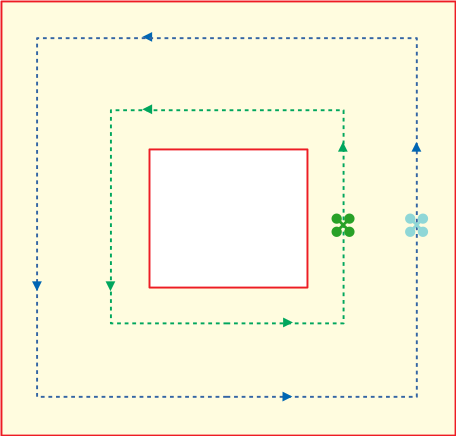
\includegraphics[width=0.9\textwidth]{normal.png}
               \end{figure}

   \section{GPS}
      \subsection{VAE trace encoding}
         \begin{figure}[H]
            \centering
            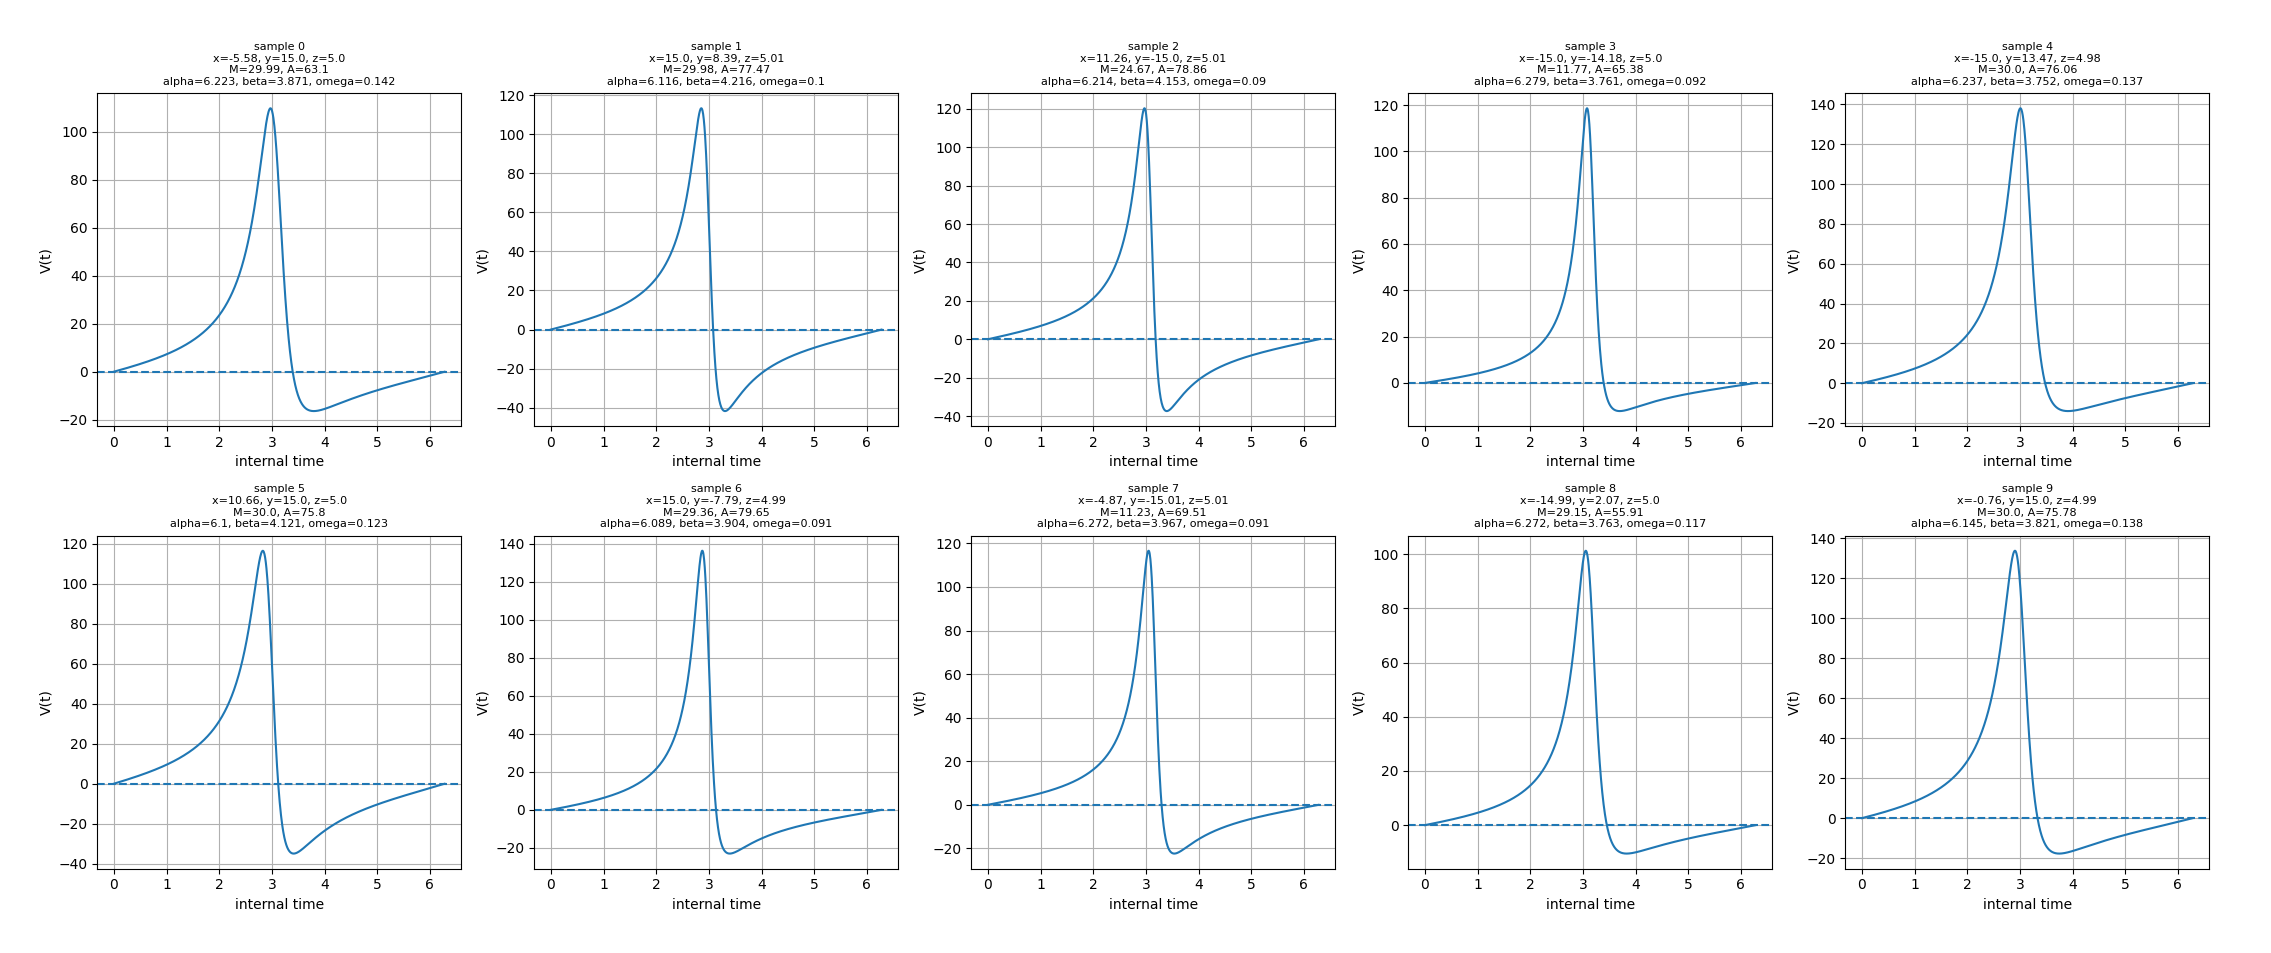
\includegraphics[width=0.9\textwidth]{gps_encoding.png}
            Here is an example of FMM waves reconstructed bay VAE from UAV1
         \end{figure}
      \subsection{Clustering}
      Here is the 0th and thes econd deriviatve of GPS (the first is wrong and must be modified)
         \begin{figure}[H]
             \centering
             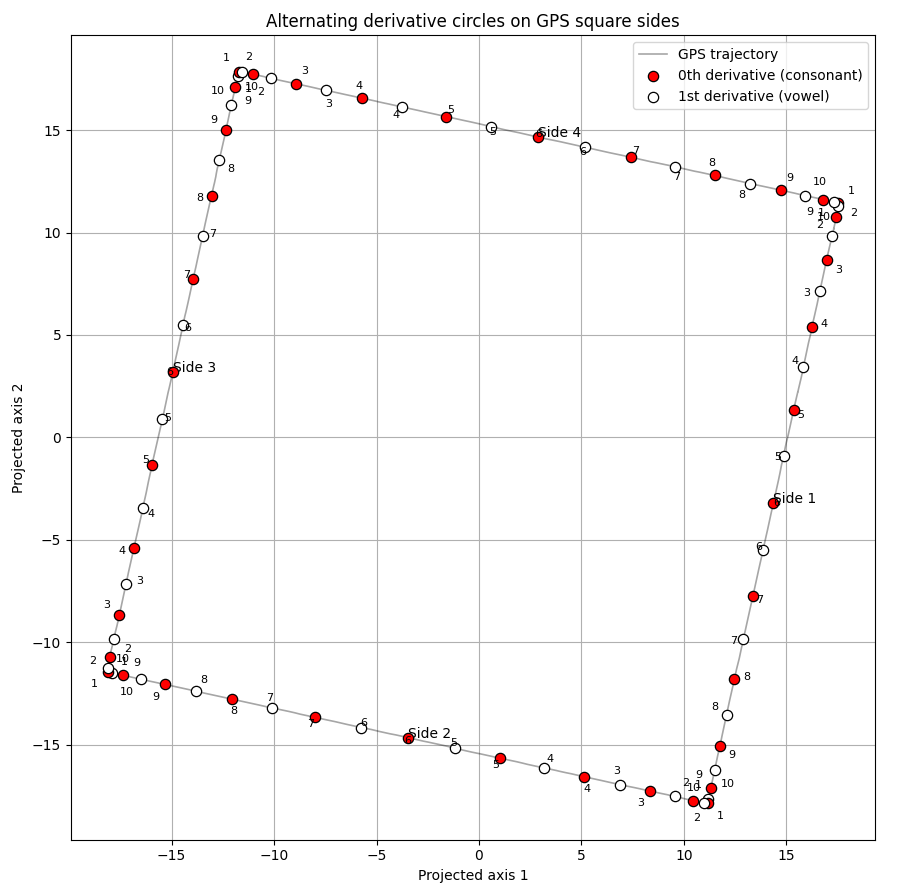
\includegraphics[width=0.9\textwidth]{gps_phonem_clustering.png}
         \end{figure}
   \section{LiDAR}

      \subsection{VAE trace encoding}
      \begin{figure}[H]
            \centering
            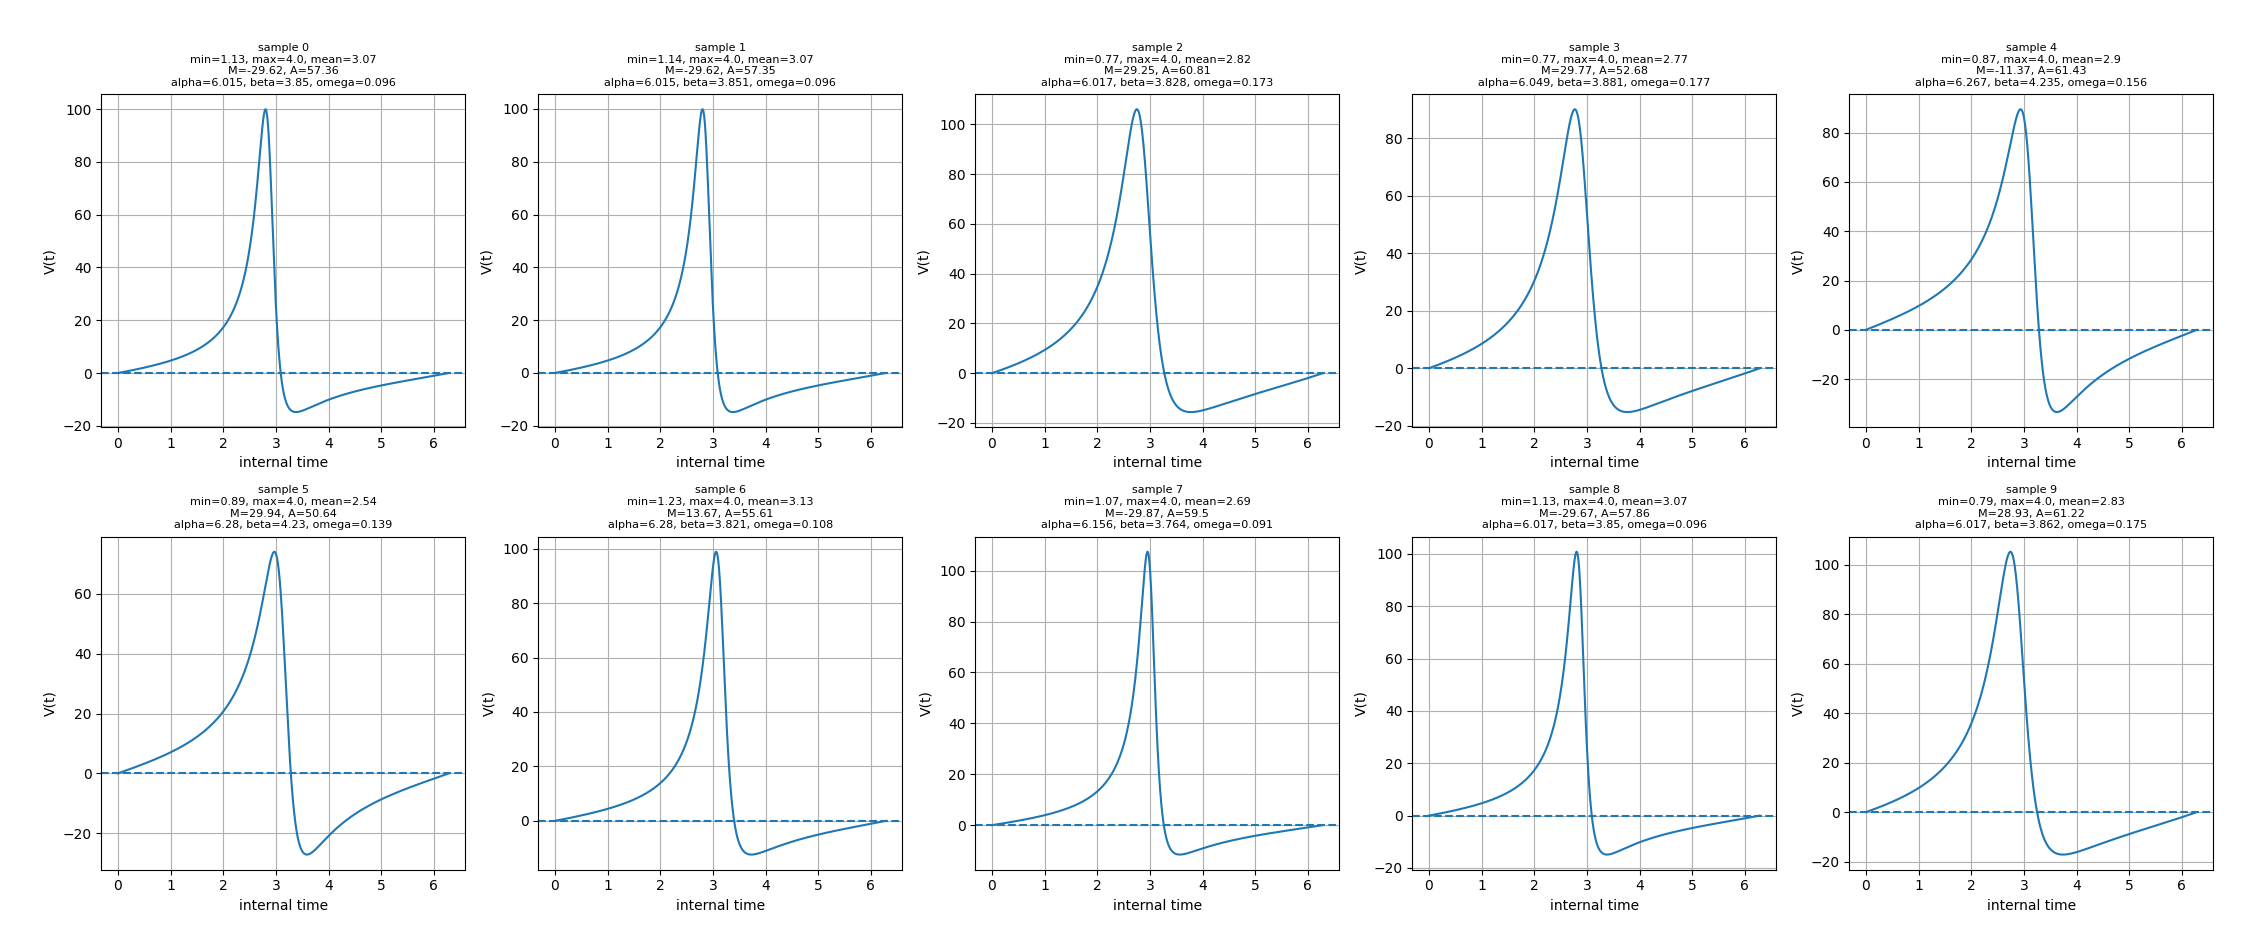
\includegraphics[width=0.9\textwidth]{lidar_encoding.png}
            Here is an example of FMM waves reconstructed bay VAE from UAV1
         \end{figure}
         \begin{figure}[H]
            \centering
            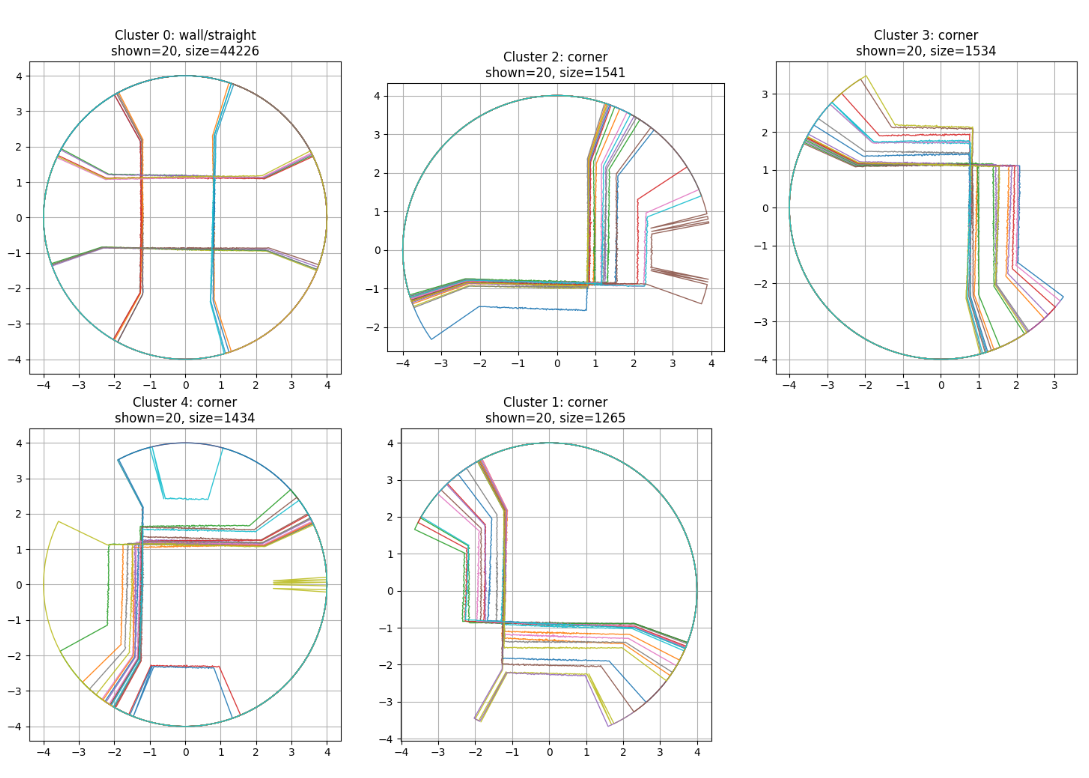
\includegraphics[width=0.9\textwidth]{clustering_lidar_zero_derivative_with_multiple_samples.png}
         \end{figure}

         Averaging members of each clster
         \begin{figure}[H]
            \centering
            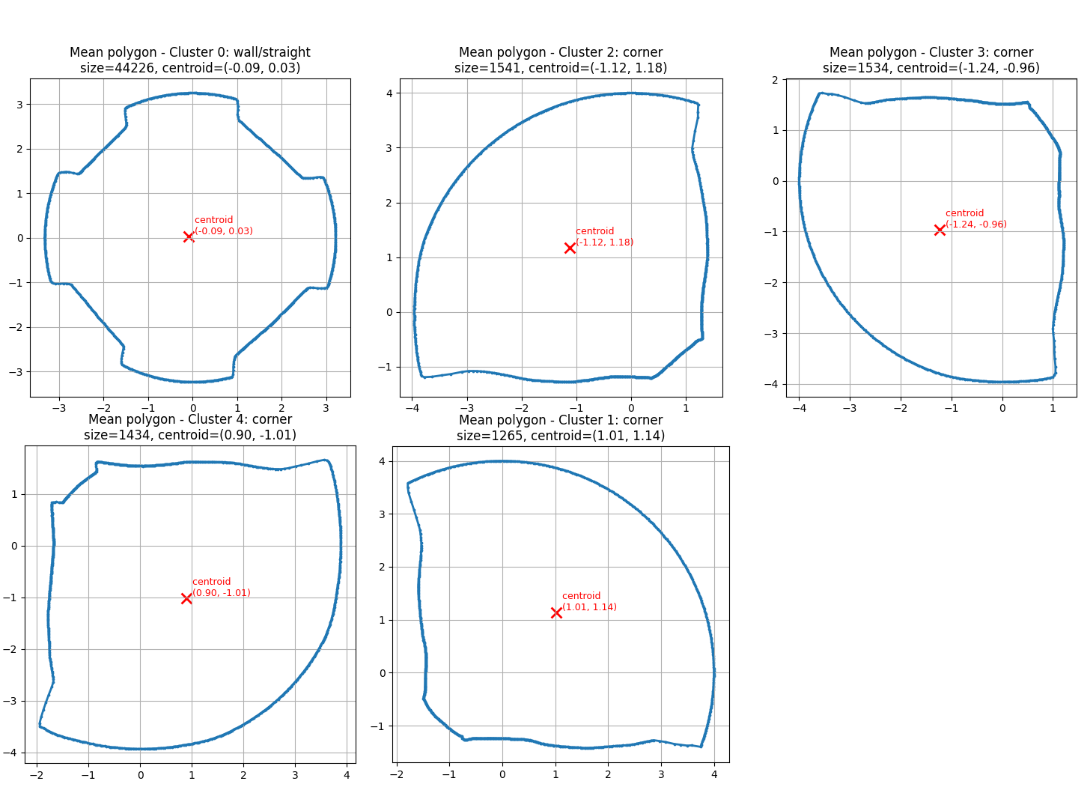
\includegraphics[width=0.9\textwidth]{clustering_lidar_zero_derivative_with_centroid.png}
         \end{figure}
         \subsection{Clustering}
         Both are for fused LiDAR and GPS
         \paragraph{Word level}
               \begin{figure}[H]
                  \centering
                  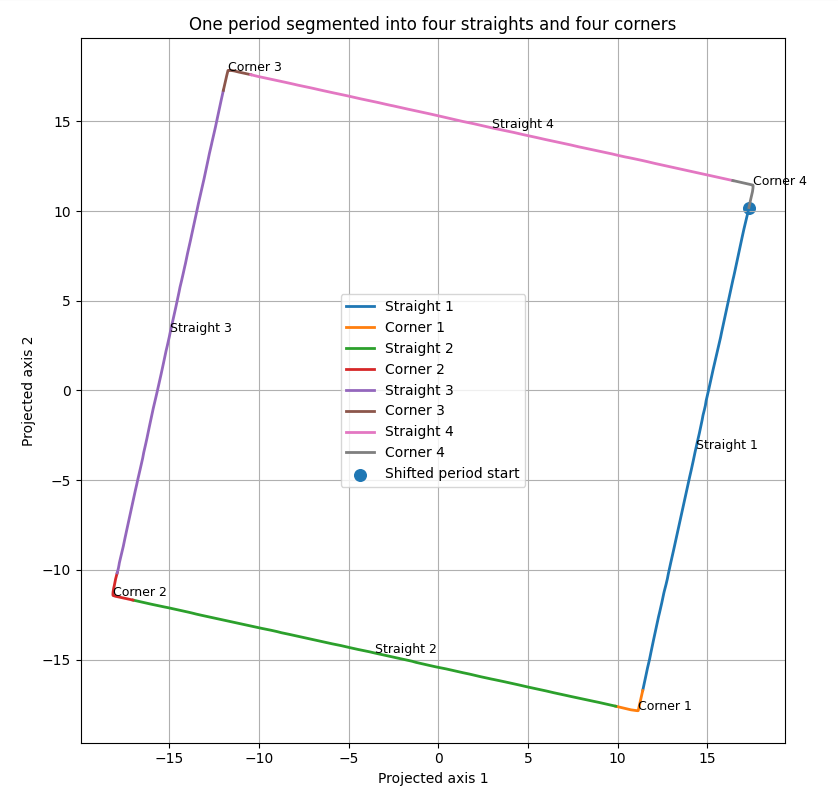
\includegraphics[width=0.9\textwidth]{word_level.png}
               \end{figure}         
         \paragraph{Senetnce level}
               \begin{figure}[H]
                  \centering
                  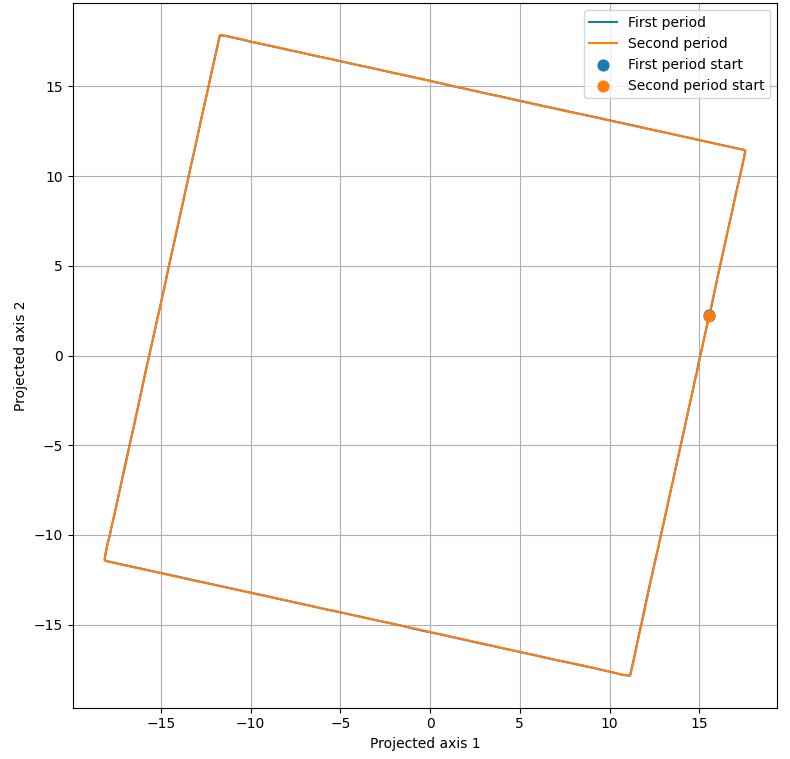
\includegraphics[width=0.9\textwidth]{sentence_level.png}
               \end{figure}
         \bibliographystyle{plainnat}
         \bibliography{/home/donkarlo/Dropbox/repo/nd_shared_research/bibliography/bibliography.bib}
\end{document}
